\documentclass{article}
\usepackage{graphicx}
\usepackage{mathtools}
\usepackage{xfrac}
\usepackage{amsmath, amssymb}
\usepackage{listings}
\usepackage{float}
\usepackage{wrapfig}
\usepackage{tikz}
\usepackage{fullpage}
\usepackage{hyperref}
\usepackage{mathalpha}
\usepackage{tikz}
\usepackage{cite}
\usepackage{amsthm}
\usepackage{natbib}
\usepackage{multirow}

\setcounter{section}{-1}

\newtheorem{theorem}{Proposition}[section]
\newtheorem{corollary}{Corollary}[theorem]
\newtheorem{lemma}[theorem]{Lemma}

\theoremstyle{definition}
\newtheorem{definition}{Definition}[section]

\theoremstyle{remark}
\newtheorem*{remark}{Remark}
\newtheorem*{example}{Example}
\newtheorem*{notation}{Notation}

\title{Fractals}
\author{David Lawton\\
        Lab Partner: Sami Lopez-Steffenson\\
        22337087}
\date{14th Oct. 2024.}

\begin{document}

\maketitle

\tableofcontents
\addcontentsline{toc}{section}{\numberline{}Abstract}
\begin{abstract}
        In this experiment, we succesfully verified several conclusions of previous papers on the subject of electrochemical deposition of zinc. The appearance and type of fractal growths were consistent with the expected behaviour, and the fractal dimensions of the homogeneous/DLA fractals at low molarity were found to be approximately $1.7$, which is in agreement with the values found in previous experiments. As well as this we observed the transition between stringy and homogeneous growths as molarity and voltage varied, as is put forward in \cite{PhysRevLett.59.2315}. \\
        \indent We also verified the accuracy of the fractal analysis software used, by analysing a straight line and a checkered pattern, with the expected answers of 1 and 2 being within reasonable distance.\\
\end{abstract}

\section{Keywords \& Preliminaries}\label{sec:keywords}
\begin{definition}
        An \textbf{`ideal' fractal} is a scale independent geometric object. Scale independent meaning that the scale on which the object is viewed does not affect the appearance.(\cite{LabHandbook})
\end{definition}
\begin{definition}
        A \textbf{`real' fractal} is a physical object which resembles a fractal one over certain scales. However, the object size sets an upper limit on the scale at which the fractal properties are observed, and of course, the resolution sets, a less defined, lower bound.(\cite{LabHandbook})
\end{definition}
\begin{definition}
        The \textbf{`fractal dimension'} of an object is a measure of it's commplexity, which is formally defined as
\begin{equation}
        \label{eq:fractal_dimension}
        D = \lim_{\varepsilon \to 0} \frac{\ln(N(\varepsilon))}{\ln(1/\varepsilon)}
\end{equation}
        where $N(r)$ is the number of units describing the object at scale $r/\varepsilon$.
\end{definition}
\begin{definition}
        \textbf{Anisotropy} measures the difference in a materials properties in different directions. If a material is isotropic, it's properties have spatial symmetry. If a material is anisotropic, it's properties do not. 
\end{definition}
\section{Background \& Theory}\label{sec:background}
This labs concerns the analysis of fractal growth under varying conditions. The fractals in this experiment were grown as described in section \ref{sec:methodology}, and then analysed using the box counting and mass-radius methods.\\
\subsection{Boxcounting \& Mass-Radius Methods}\label{sec:fractalmethods}
\indent The \textbf{box counting method} is a standard way of estimating fractal dimension. It involves covering the fractal with a mesh of mesh size $s = w/\varepsilon$, where $w$ is the width of the fractal and $\varepsilon$ is a scaling factor. The number of boxes $N(s)$ which contain part of the fractal is then counted. This is done for many values of $s$, until the boxes of a size such that they cannot be reduced further (pixel size) are reached. The fractal dimension is estimated by fitting a line to the graph of $\ln(N(s))$ against $\ln(s)$. The line is of the form
\begin{equation}
        \ln(N(\varepsilon)) = m\ln(s) + c
\end{equation}
We recall Eq. \ref{eq:fractal_dimension} and solve for $D=-m$ to find the fractal dimension.\\
\indent The \textbf{mass-radius method} is another method of estimating the fractal dimension of an object. A centre of the fractal is identified, and then a series of squares (for raster data) of width $r$ are placed centred on that point, with many values of $r$ taken, the area of the structure inside each square is recorded, and $\ln(N(r))$ is plotted against $r$, and the dimension is found to be the slope of the linear fit to this plot. One problem found with this method is that the lines produced are not really linear. This is because the area around the centre is usually filled (giving slope 2 initially), and the slope goes to zero as the square passes the bounds of the fractal. The solution found was to take into account only the $r$ values for which neither of these sections were considered, for the most part, as in figure \ref{fig:radiuscutting} (a)\\
\begin{figure}[H]
        \begin{tabular}{cc}
                \centering
                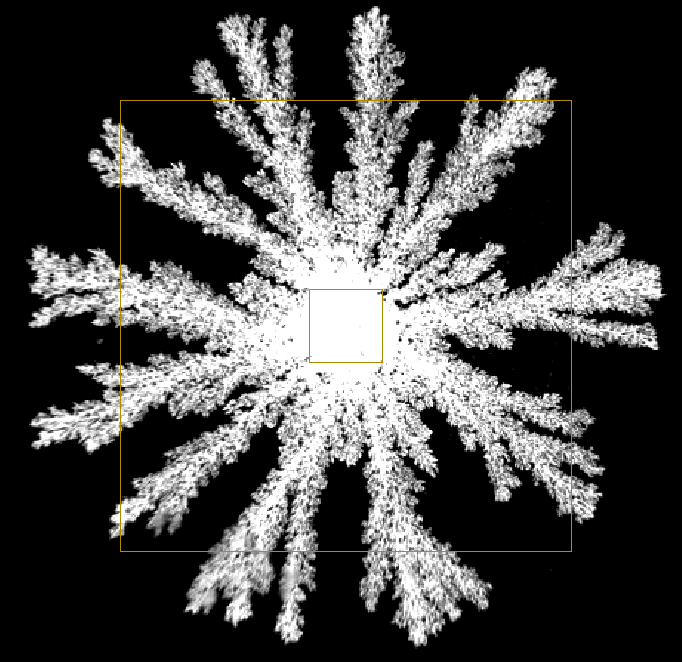
\includegraphics[width=0.5\textwidth]{radius_cutting_img.png} & 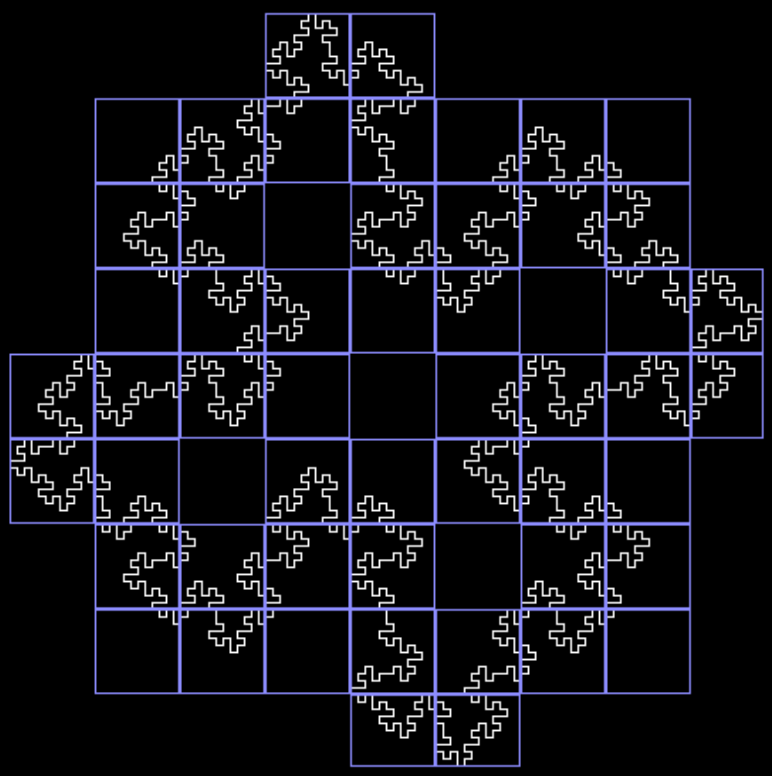
\includegraphics[width=0.5\textwidth]{Boxcounting.png}\\
                (a) & (b)
        \end{tabular}
        \caption{\label{fig:radiuscutting}Illustration of the dimension estimation methods. (a) Shows the effect of varying included $r$ values, as indicated by the thin yellow lines, in the mass-radius method. Note that they are chosen such that the area of the filled centre and outer empty area inside the considered zone are minimised. (b)(\cite{ImageJ}) Shows an example of the box counting method, where the fractal is covered by a mesh of boxes of size $s$.}
\end{figure}

\subsection{Fractal Classifications}\label{sec:fractalclassifications}
\indent In our analysis we categorise our fractals as in \cite{PhysRevLett.56.1260}, in four categories, however we also include Diffusion-limited Aggregation (DLA) as a fifth category, as structures of this type are not easily described by the other four.:
\begin{enumerate}
        \item \textbf{Stringy} - Fractals which are made up of long thin branches. (Figure \ref{fig:fractal types} (a))
        \item \textbf{Open} - Thick open ramified structures that, while fractal, dont show particularly fine structure, nor do they show any particular symmetry. (Figure \ref{fig:fractal types} (b))
        \item \textbf{Dendritic} - Many large branches, with similar smaller branches offshooting, significant fractal behaviour and self similarity. (Figure \ref{fig:fractal types} (c))
        \item \textbf{Homogeneous} - In these fractals, the zinc deposits spread uniformly over the cathode, and the fractal dimension closer to 2. (Figure \ref{fig:fractal types} (d))
        \item \textbf{Diffusion-limited Aggregation (DLA)} - Fractal growths which are not self-similar, outlined in \cite{1981PhRvL..47.1400W}. Although should have general circular symmetry, as the example in figure \ref{fig:DLA}.
\end{enumerate}
\begin{figure}[H]
        \centering
        \begin{tabular}{cc}
                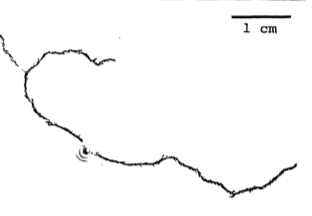
\includegraphics[width=0.4\textwidth]{Stringy_fractal.png} & 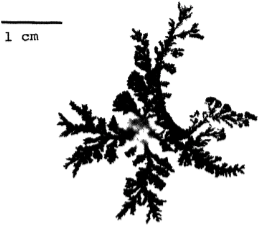
\includegraphics[width=0.4\textwidth]{Open_fractal'.png}\\
                (a) & (b)\\
                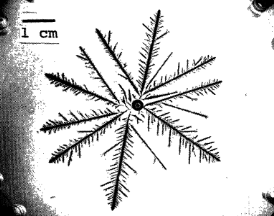
\includegraphics[width=0.4\textwidth]{Dendritic_fractal.png} & 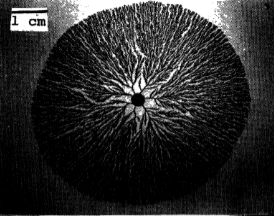
\includegraphics[width=0.4\textwidth]{Homogeneous_fractal.png}\\
                (c) & (d)
        \end{tabular}
        \caption{\label{fig:fractal types}Examples of the four classifications of fractals used in this experiment. (a) Stringy: Little fractal behaviour, very fast growth; (b) Open; fractal on a local scale, but lack of defined general symmetry (c) Dendritic: Evident fractal pattern and scale independence; (d) Homogeneous: Evenly spread, circularly symmetrical, described in \cite{PhysRevLett.56.1260} as being due to tip-splitting instability.}
\end{figure}
\begin{figure}
        \centering
        \includegraphics[width=0.5\textwidth]{fractal images/Fractals_25M_3V.jpg}
        \caption{\label{fig:DLA} An example of fractal which we produced, that can be described by diffusion-limited aggregation. Note the large amounts of tip-splitting, and lack of central growth. \cite{1981PhRvL..47.1400W} explains the lack of central growth as being due to the more central sites being `shadowed' by outer structures.}
\end{figure}

\subsection{Physical Theory}\label{sec:physicaltheory}
It is of course important to discuss the fashion in which the fractals grow. In this experiment, the fractals grow due to the $Zn^{2+}$ ions from the zinc sulphate monohydrate solution diffusing toward the cathode. This happens due to the electric field between the cathode and anode, generated by the voltage applied across the solution. These $Zn^{2+}$ ions are deposited on the cathode (graphite), becoming a part of the cathode, this is called electrochemical deposition. The fractal growth is due to the continual deposition of these ions, on the graphite and each other. As is described in \cite{PhysRevLett.59.2315}, the nature of this growth changes significantly with the anisotropy of the crystal structure of the zinc deposits. At large values of $V$, or $M$, the crystal structure has a more anisotropic structure, and so the macroscopic structure is more stable, with less tip-splitting, such as the `dendritic' or `stringy' growths. \\
\indent At lower values of $V$ or $M$, the crystal structure is more isotropic, and so growth is more evenly distributed due to increased instability, i.e. more tip-splitting. This leads to the homogeneous and DLA structures observed.\\
\begin{figure}[H]
        \centering
        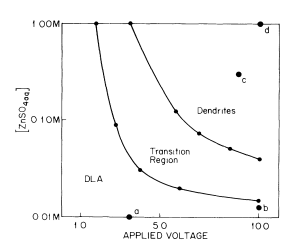
\includegraphics[width=0.5\textwidth]{GrieretalFractaltransition.png}
        \caption{\label{fig:fractal transition}The transition from stringy and dendritic growth to homogeneous and DLA growth as molarity and voltage vary. Given the similar range of voltages considered, we expect our results to agree with this. \cite{PhysRevLett.59.2315}}
\end{figure}




\section{Methodology}\label{sec:methodology}
\textbf{A sketch of the experimental setup can be found in figure \ref{fig:Sketch} in the appendix.}\\
The procedure of this experiment begins with the preparation of the zinc sulphate monohydrate solution. We first find the molar mass of zinc sulphate monohydrate, which has the formula $ZnSO_4H_2O$.
\begin{align*}
        M_{ZnSO_4H_2O} &= M_{Zn} + M_{S} + 4M_{O} + 2M_{H} + M_{O} = 65\\
        M_{ZnSO_4H_2O} &= 65.38 + 32.066 + 4(16.000) + 2(1.008) + 16.000 = 179.462\text{ g/mol}
\end{align*}
We then make samples of concentrations 1M, 0.25M, 0.1M and 0.01M, by first making $200$ml of 1M solution ($200ml$ deionised water, $39.892g$ of $ZnSO_4H_2O$), and then diluting appropriately with deionised water.
\indent While making the 1M solution balance was used to measure the volume of water and mass of $ZnSO_4H_2O$. The $ZnSO_4H_2O$ was ground in a pestle and mortar to remove clumps from the powder, and then added slowly to the water, stirring continuously to ensure a homogeneous solution without undisolved $ZnSO_4H_2O$ remaining. When diluting further some of this solution, measurements were taken using a $50ml$ lab syringe, and mixing in a beaker with an aappropriate amount of deionised water.\\
\indent The configuration of the experiment was similar to that in (\cite{PhysRevLett.56.1260}), where the solution is placed in a very shallow cylindrical gap between a plexiglass plate, and a disk fitting into the gap (note that care must be taken to avoid bubbles forming in the solution), with a conducting ring on the edge, and a graphite stick entering through a hole in the centre of the upper disk. Both the ring and the stick are connected to a power supply, with the graphite acting as the cathode and ring as the anode. The voltage across the solution is kept constant, and the zinc from the $ZnSO_4H_2O$ deposits on the cathode, becoming a part of it. The fractal growth due to this continual deposition is then observed and recorded.\\
\indent The fractal growth is recorded using a camera, and while usually in this experiment, the lab software ImageJ and Benoit would be used to manipulate the images and analyse the fractals respectively, in this case, due to time constraints, these tasks were instead done using GNU Image Manipulation Program and Fractalyse, a fractal analysis software written in java which can be found \href{https://sourcesup.renater.fr/www/fractalyse/}{here}. I would recommend the use of this software, as it is very user friendly, and has a lot of features which are useful for the analysis of fractals.\\
\indent Both the box counting and the mass-radius methods (outlined in \ref{sec:background}) of fractal analysis were used in this experiment to find the fractal dimensions of the samples, and each growth was given approximate classification of 1 or 2 types.
\section{Results}
The results of the analysis of the collected fractals by the previously outlined methods (section \ref{sec:fractalmethods}) are shown in the tables below. The fractals were classified as in section \ref{sec:fractalclassifications}, and the images of the fractals are shown in figure \ref{fig:fractal images} below.\\
\indent The general increase of fractal dimension with decreasing molarity is clear, and expected. However, one would expect more DLA behaviour at low molarity, as well as more radial behaviour in the `transitionary' region between the stringy and homogeneous growths. As well as this very little true dendritic behaviour, as in figure \ref{fig:fractal types} (c), was observed. This is not truly unexpected however, since these only grow in a narrow region (\cite{PhysRevLett.56.1260}).\\
\begin{center}
\begin{tabular}{|l|l||l|l|l||l|l|l||l|}
        \hline
            $M$ & $V\pm0.1$ & $D_m$ & \multicolumn{2}{c|}{$D_m$ Confidence} & $D_b$ & \multicolumn{2}{c|}{$D_b$ Confidence} & Type \\ \hline
            $1.000\pm0.001$ & 7 & 1.203 & 1.125 & 1.281 & 1.290 & 1.259 & 1.321 & Stringy/Dendritic \\ \hline
            $1.000\pm0.001$ & 5 & 1.111 & 1.088 & 1.133 & 1.339 & 1.301 & 1.377 & Stringy \\ \hline
            $1.000\pm0.001$ & 3 & 1.099 & 1.060 & 1.138 & 1.313 & 1.271 & 1.355 & Stringy \\ \hline
            $0.251\pm0.028$ & 7 & 1.696 & 1.623 & 1.769 & 1.486 & 1.444 & 1.527 & Stringy/Open \\ \hline
            $0.251\pm0.028$ & 5 & 1.423 & 1.390 & 1.456 & 1.490 & 1.462 & 1.519 & Open/Dendritic \\ \hline
            $0.251\pm0.028$ & 3 & 1.749 & 1.599 & 1.898 & 1.537 & 1.515 & 1.558 & DLA \\ \hline
            $0.100\pm0.001$ & 7 & 1.621 & 1.550 & 1.692 & 1.527 & 1.494 & 1.561 & Open/Stringy \\ \hline
            $0.100\pm0.001$ & 5 & 1.337 & 1.256 & 1.419 & 1.483 & 1.439 & 1.534 & Dendritic/Stringy \\ \hline
            $0.100\pm0.001$ & 3 & 1.595 & 1.533 & 1.656 & 1.534 & 1.522 & 1.546 & DLA \\ \hline
            $0.010\pm0.001$ & 7 & 1.815 & 1.768 & 1.862 & 1.793 & 1.773 & 1.812 & Homogenous/DLA \\ \hline
            $0.010\pm0.001$ & 5 & 1.748 & 1.688 & 1.809 & 1.712 & 1.695 & 1.728 & Homogeneous/DLA \\ \hline
            $0.010\pm0.001$ & 3 & 1.854 & 1.811 & 1.909 & 1.673 & 1.647 & 1.699 & Homogeneous/DLA \\ \hline
\end{tabular}
\end{center}
There are significant differences in the measured fractal dimensions between the two methods. This is expected, since the mass-radius method can be altered to not account for the thick central areas of the fractal, as in \ref{fig:radiuscutting}. The box counting method however does provide a dimension more consistent to the entire structure.\\
\indent One notable inconsistency from prior experiments is the dip in fractal dimension at the $5V$ mark of the $0.1M$ and $0.25M$ samples. The expected behaviour from \cite{PhysRevLett.59.2315} would be a marked increase in fractal dimension in this region.\\
\indent We next observe how the behaviour changes with molarity and voltage, as it corresponds to growth type. The sample at $0.1M$, $5V$ is a clear outlier from the expected behaviour, as we would expect a more homogeneous growth for these values of molarity and voltage (figure \ref{fig:fractal transition}).\\
\begin{center}
\begin{tabular}{|ll|l|l|l|}
        \hline
             ~& ~& \multicolumn{3}{c|}{Voltage ($V$)} \\ \cline{3-5}
             ~& ~& 3 & 5 & 7 \\ \hline
            \multirow{4}{*}{Molarity ($M$)} & $1.000\pm0.001$ & Stringy & Stringy & Stringy/Dendritic \\
            & $0.251\pm0.028$ & DLA & Open/Dendritic & Open/Stringy \\     
            & $0.100\pm0.001$ & DLA & Stringy/Open? & Open/Stringy \\
            & $0.010\pm0.001$ & Homogeneous/DLA & Homogeneous/DLA & Homogeneous/DLA \\ \hline
 \end{tabular}
\end{center}
For the most part however, the results are consistent with previous experiments. Low molarities and voltages lead, in general, to more dense, evenly spread growth, while higher molarities and voltages lead to more stringy, dendritic growth. In figure \ref{fig:fractal images}, there is a clear visual transition from the  more homogeneous types of growth to the more simple, one-dimensional types, although once again the $0.1M$, $5V$ sample is an outlier.\\
\begin{figure}[H]
        \centering
        \begin{tabular}{|ll|l|l|l|}
        \hline
             ~& ~& \multicolumn{3}{c|}{Voltage ($V$) $\pm0.1$} \\ \cline{3-5}
             ~& ~& 3 & 5 & 7 \\ \hline
            \multirow{4}{*}{Molarity ($M$)} & $1.000\pm0.001$ & 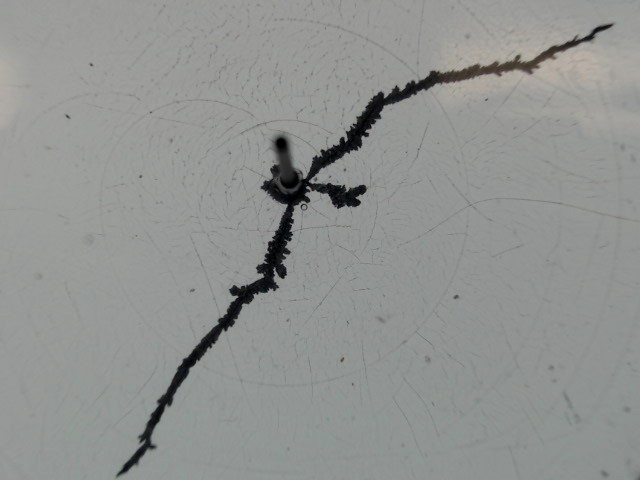
\includegraphics[width=0.25\textwidth]{/home/dj-lawton/Documents/Junior Sophister/JS Labs/Fractals/fractal images/Fractal1M3V_Light3.jpg} & 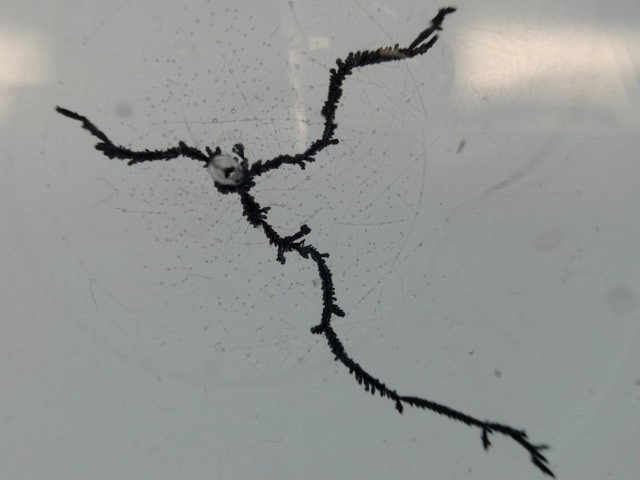
\includegraphics[width=0.25\textwidth]{/home/dj-lawton/Documents/Junior Sophister/JS Labs/Fractals/fractal images/Fractal1M5V_Light0.jpg} & 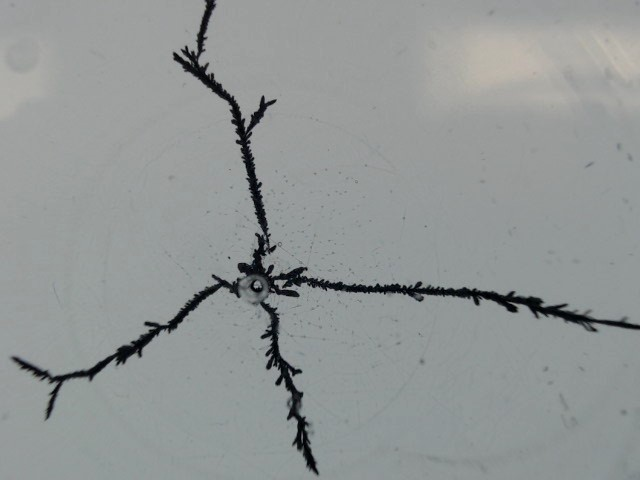
\includegraphics[width=0.25\textwidth]{/home/dj-lawton/Documents/Junior Sophister/JS Labs/Fractals/fractal images/Fractal1M7V_Light3.jpg} \\ \cline{2-5}
            & $0.251\pm0.028$ & \includegraphics[width=0.25\textwidth]{/home/dj-lawton/Documents/Junior Sophister/JS Labs/Fractals/fractal images/Fractals_25M_3V} & 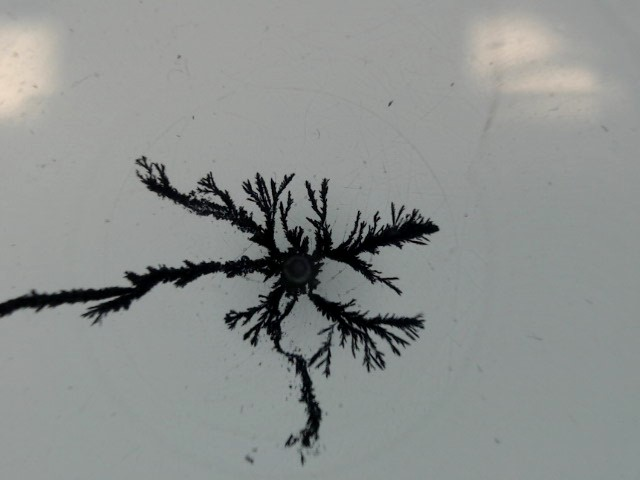
\includegraphics[width=0.25\textwidth]{/home/dj-lawton/Documents/Junior Sophister/JS Labs/Fractals/fractal images/Fractals_0.25M_5V.jpg} & 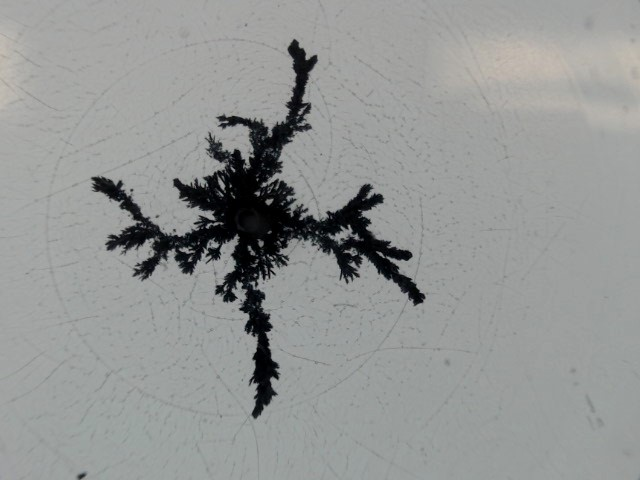
\includegraphics[width=0.25\textwidth]{/home/dj-lawton/Documents/Junior Sophister/JS Labs/Fractals/fractal images/Fractal25M7V_light3.jpg} \\     \cline{2-5}
            & $0.100\pm0.001$ & 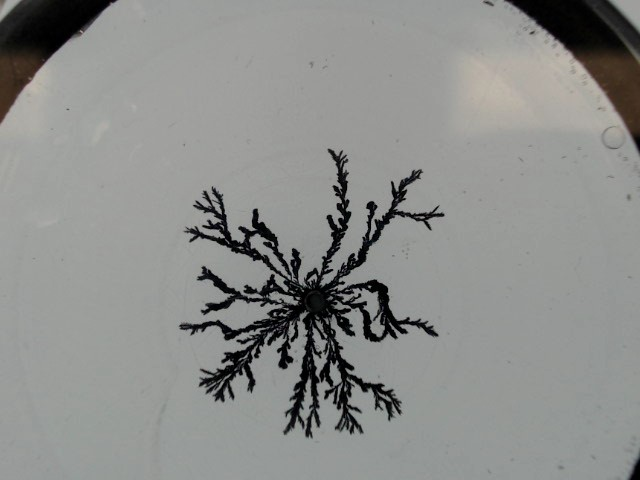
\includegraphics[width=0.25\textwidth]{/home/dj-lawton/Documents/Junior Sophister/JS Labs/Fractals/fractal images/Fractals_0.1M_3V.jpg} & 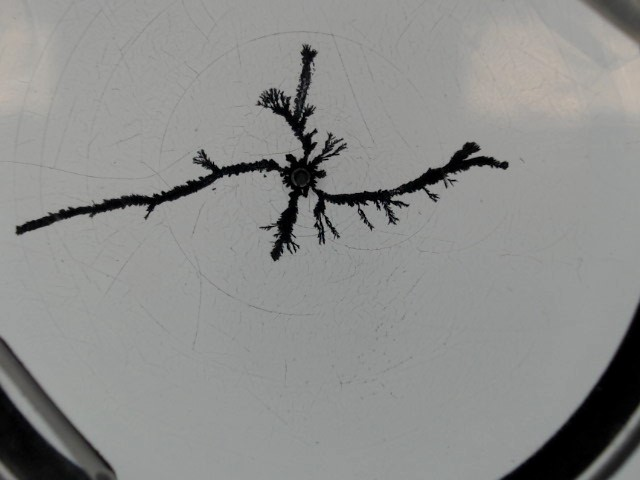
\includegraphics[width=0.25\textwidth]{//home/dj-lawton/Documents/Junior Sophister/JS Labs/Fractals/fractal images/Fractals_0.1M_5V.jpg} & 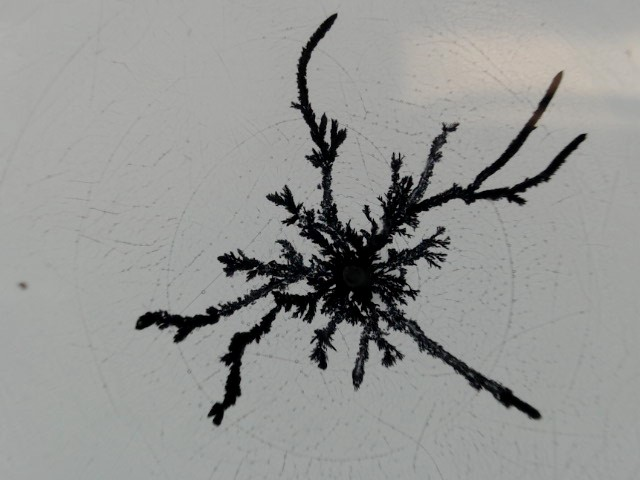
\includegraphics[width=0.25\textwidth]{/home/dj-lawton/Documents/Junior Sophister/JS Labs/Fractals/fractal images/Fractals_0.1M_7V.jpg} \\ \cline{2-5}
            & $0.010\pm0.001$ & 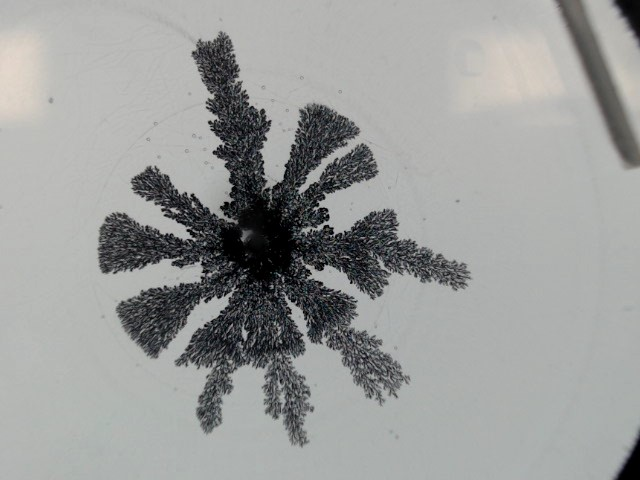
\includegraphics[width=0.25\textwidth]{/home/dj-lawton/Documents/Junior Sophister/JS Labs/Fractals/fractal images/Fractals_0.01M_3V.jpg} & 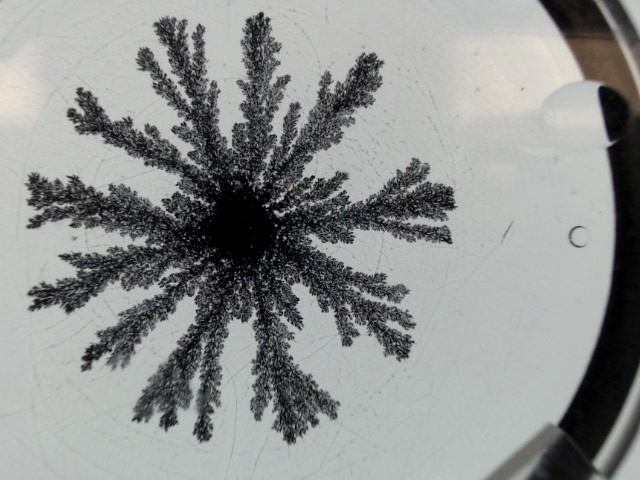
\includegraphics[width=0.25\textwidth]{/home/dj-lawton/Documents/Junior Sophister/JS Labs/Fractals/fractal images/Fractals0.01M5V.jpg} & 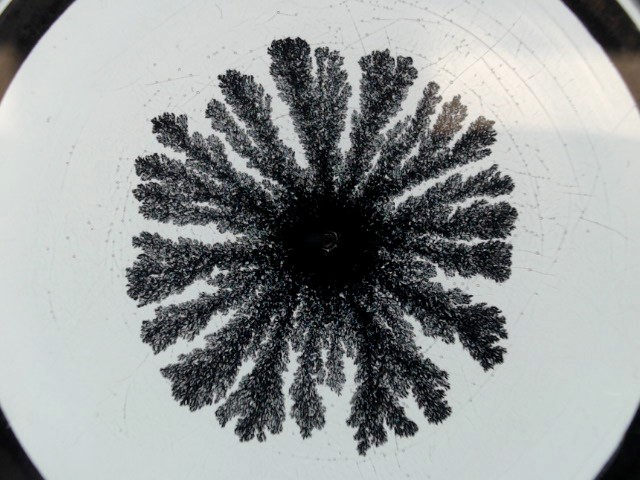
\includegraphics[width=0.25\textwidth]{/home/dj-lawton/Documents/Junior Sophister/JS Labs/Fractals/fractal images/Fractals_0.01M_7V.jpg} \\ \hline
        \end{tabular}
        \caption{\label{fig:fractal images}Images of the fractals produced in this experiment. The shift from stringy to more evenly spread growth is evident as both molarity and voltage decrease.}
\end{figure}
To verify the accuracy of the fractal analysis, we analyse a straight line (1D), and a checkered pattern (2D), and find the expected fractal dimensions of 1 and 2 respectively. The results are shown in the table below.\\
\begin{center}
        \begin{tabular}{|c|c|c|c|c|}
                \hline
                Sample & $D_b$ & $D_m$ & $D_b$ Confidence & $D_m$ Confidence \\ \hline
                1D & 0.9919 & 1.021 & [0.9066 - 1.077] & [1.003 - 1.040]\\ \hline
                2D & 1.903 & 2.009 & [1.823 - 1.984] & [2.002 - 2.017] \\ \hline
        \end{tabular}
\end{center}
This indicates that while most of these have the expected dimension inside the confidence interval, the box dimension is perhaps not properly calibrated.
\section{Discussion}
In this experiment we verified much of the results and theory of previous descriptions of electrochemical deposition of zinc. And while the results were mostly consistent with the expected behaviour, there were definitely parts of this experiment which could have been executed more effectively. For instance, monitoring of voltage across the solution, as well as the depth of the solution, would have been useful in more precisely pinpointing the conditions under which each fractal was grown.\\
\indent The results at low molarity especially were consistent with theory, as the box dimensions of the dense, evenly spread growths at $0.01M$ were approx. 1.7, as expected (\cite{1981PhRvL..47.1400W}, \cite{PhysRevLett.59.2315}). It also grew as $V$ increased, toward the transition region, as observed in \cite{PhysRevLett.59.2315}.\\
\indent Other approaches which could be considered would be multi-fractal analysis, which is a technique that takes into account not only the presence of the fractal behaviour, but the distibution of fractal behaviours present, or correlation dimension, as is used in \cite{1981PhRvL..47.1400W}. Of course on repetition one would gather a larger sample size for more definite results. \\


\bibliographystyle{plainnat}
\bibliography{references}

\addcontentsline{toc}{section}{\numberline{}Appendix}
\section*{Appendix}\label{sec:appendix}
All images, data and code used in this experiment can be found \href{https://github.com/DavidLawton04/MuchStuff/tree/0e61b8d6692b4b1c47f4bab8d9bb8fb7e5c122d6/Junior%20Sophister/JS%20Labs/Fractals}{here}.

\begin{figure}[H]
        \centering
        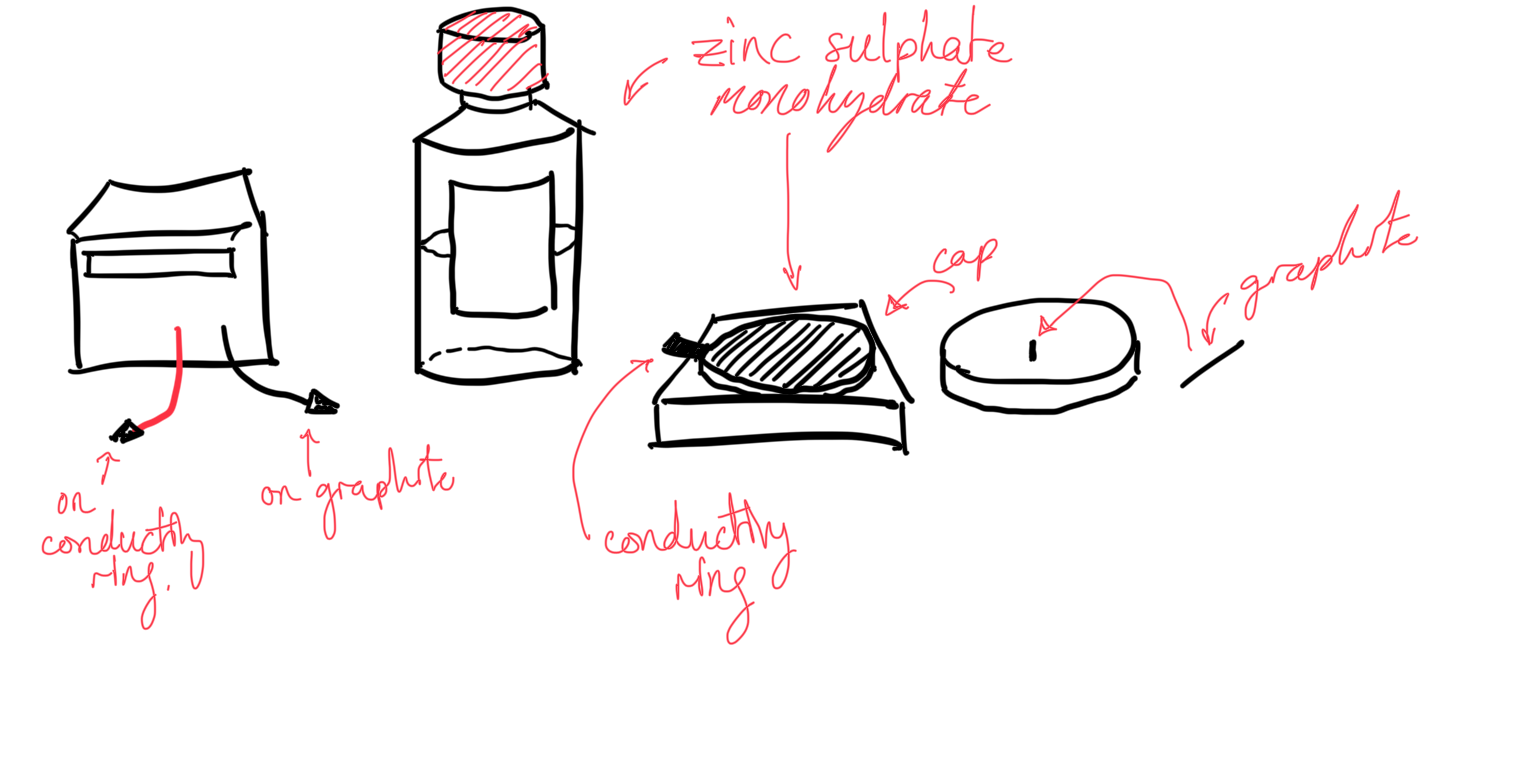
\includegraphics[width=0.5\textwidth]{FractalsSketch.png}
        \caption{\label{fig:Sketch} Sketch of the experimental setup. The solution is placed in the gap between the plexiglass plate and the disk, with the graphite stick entering through the hole in the centre of the disk. The ring around the edge of the disk is connected to the red cable, and the graphite to the black cable}
\end{figure}


\end{document}